\documentclass{article}

\usepackage{hyperref}
\hypersetup{
	colorlinks=true,
	linkcolor=blue,
	urlcolor=cyan,}
\usepackage{booktabs}
\usepackage{textgreek}

%%%%%%%%%%%%%%%%%%%%%%%%%%%%%%%%%%%%%%%%%
% Lachaise Assignment
% Structure Specification File
% Version 1.0 (26/6/2018)
%
% This template originates from:
% http://www.LaTeXTemplates.com
%
% Authors:
% Marion Lachaise & François Févotte
% Vel (vel@LaTeXTemplates.com)
%
% License:
% CC BY-NC-SA 3.0 (http://creativecommons.org/licenses/by-nc-sa/3.0/)
% 
%%%%%%%%%%%%%%%%%%%%%%%%%%%%%%%%%%%%%%%%%

%----------------------------------------------------------------------------------------
%	PACKAGES AND OTHER DOCUMENT CONFIGURATIONS
%----------------------------------------------------------------------------------------

\usepackage{amsmath,amsfonts,stmaryrd,amssymb} % Math packages

\usepackage{enumerate} % Custom item numbers for enumerations

\usepackage[ruled]{algorithm2e} % Algorithms

\usepackage[framemethod=tikz]{mdframed} % Allows defining custom boxed/framed environments

\usepackage{listings} % File listings, with syntax highlighting
\lstset{
	basicstyle=\ttfamily, % Typeset listings in monospace font
}

%----------------------------------------------------------------------------------------
%	DOCUMENT MARGINS
%----------------------------------------------------------------------------------------

\usepackage{geometry} % Required for adjusting page dimensions and margins

\geometry{
	paper=a4paper, % Paper size, change to letterpaper for US letter size
	top=2.5cm, % Top margin
	bottom=3cm, % Bottom margin
	left=2.5cm, % Left margin
	right=2.5cm, % Right margin
	headheight=14pt, % Header height
	footskip=1.5cm, % Space from the bottom margin to the baseline of the footer
	headsep=1.2cm, % Space from the top margin to the baseline of the header
	%showframe, % Uncomment to show how the type block is set on the page
}

%----------------------------------------------------------------------------------------
%	FONTS
%----------------------------------------------------------------------------------------

\usepackage[utf8]{inputenc} % Required for inputting international characters
\usepackage[T1]{fontenc} % Output font encoding for international characters

\usepackage{XCharter} % Use the XCharter fonts

%----------------------------------------------------------------------------------------
%	COMMAND LINE ENVIRONMENT
%----------------------------------------------------------------------------------------

% Usage:
% \begin{commandline}
%	\begin{verbatim}
%		$ ls
%		
%		Applications	Desktop	...
%	\end{verbatim}
% \end{commandline}

\mdfdefinestyle{commandline}{
	leftmargin=10pt,
	rightmargin=10pt,
	innerleftmargin=15pt,
	middlelinecolor=black!50!white,
	middlelinewidth=2pt,
	frametitlerule=false,
	backgroundcolor=black!5!white,
	frametitle={Command Line},
	frametitlefont={\normalfont\sffamily\color{white}\hspace{-1em}},
	frametitlebackgroundcolor=black!50!white,
	nobreak,
}

% Define a custom environment for command-line snapshots
\newenvironment{commandline}{
	\medskip
	\begin{mdframed}[style=commandline]
}{
	\end{mdframed}
	\medskip
}

%----------------------------------------------------------------------------------------
%	FILE CONTENTS ENVIRONMENT
%----------------------------------------------------------------------------------------

% Usage:
% \begin{file}[optional filename, defaults to "File"]
%	File contents, for example, with a listings environment
% \end{file}

\mdfdefinestyle{file}{
	innertopmargin=1.6\baselineskip,
	innerbottommargin=0.8\baselineskip,
	topline=false, bottomline=false,
	leftline=false, rightline=false,
	leftmargin=2cm,
	rightmargin=2cm,
	singleextra={%
		\draw[fill=black!10!white](P)++(0,-1.2em)rectangle(P-|O);
		\node[anchor=north west]
		at(P-|O){\ttfamily\mdfilename};
		%
		\def\l{3em}
		\draw(O-|P)++(-\l,0)--++(\l,\l)--(P)--(P-|O)--(O)--cycle;
		\draw(O-|P)++(-\l,0)--++(0,\l)--++(\l,0);
	},
	nobreak,
}

% Define a custom environment for file contents
\newenvironment{file}[1][File]{ % Set the default filename to "File"
	\medskip
	\newcommand{\mdfilename}{#1}
	\begin{mdframed}[style=file]
}{
	\end{mdframed}
	\medskip
}

%----------------------------------------------------------------------------------------
%	NUMBERED QUESTIONS ENVIRONMENT
%----------------------------------------------------------------------------------------

% Usage:
% \begin{question}[optional title]
%	Question contents
% \end{question}

\mdfdefinestyle{question}{
	innertopmargin=1.2\baselineskip,
	innerbottommargin=0.8\baselineskip,
	roundcorner=5pt,
	nobreak,
	singleextra={%
		\draw(P-|O)node[xshift=1em,anchor=west,fill=white,draw,rounded corners=5pt]{%
		Question \theQuestion\questionTitle};
	},
}

\newcounter{Question} % Stores the current question number that gets iterated with each new question

% Define a custom environment for numbered questions
\newenvironment{question}[1][\unskip]{
	\bigskip
	\stepcounter{Question}
	\newcommand{\questionTitle}{~#1}
	\begin{mdframed}[style=question]
}{
	\end{mdframed}
	\medskip
}

%----------------------------------------------------------------------------------------
%	WARNING TEXT ENVIRONMENT
%----------------------------------------------------------------------------------------

% Usage:
% \begin{warn}[optional title, defaults to "Warning:"]
%	Contents
% \end{warn}

\mdfdefinestyle{warning}{
	topline=false, bottomline=false,
	leftline=false, rightline=false,
	nobreak,
	singleextra={%
		\draw(P-|O)++(-0.5em,0)node(tmp1){};
		\draw(P-|O)++(0.5em,0)node(tmp2){};
		\fill[black,rotate around={45:(P-|O)}](tmp1)rectangle(tmp2);
		\node at(P-|O){\color{white}\scriptsize\bf !};
		\draw[very thick](P-|O)++(0,-1em)--(O);%--(O-|P);
	}
}

% Define a custom environment for warning text
\newenvironment{warn}[1][Warning:]{ % Set the default warning to "Warning:"
	\medskip
	\begin{mdframed}[style=warning]
		\noindent{\textbf{#1}}
}{
	\end{mdframed}
}

%----------------------------------------------------------------------------------------
%	INFORMATION ENVIRONMENT
%----------------------------------------------------------------------------------------

% Usage:
% \begin{info}[optional title, defaults to "Info:"]
% 	contents
% 	\end{info}

\mdfdefinestyle{info}{%
	topline=false, bottomline=false,
	leftline=false, rightline=false,
	nobreak,
	singleextra={%
		\fill[black](P-|O)circle[radius=0.4em];
		\node at(P-|O){\color{white}\scriptsize\bf i};
		\draw[very thick](P-|O)++(0,-0.8em)--(O);%--(O-|P);
	}
}

% Define a custom environment for information
\newenvironment{info}[1][Info:]{ % Set the default title to "Info:"
	\medskip
	\begin{mdframed}[style=info]
		\noindent{\textbf{#1}}
}{
	\end{mdframed}
}
 % Include the file specifying the document structure and custom commands

%----------------------------------------------------------------------------------------
%	ASSIGNMENT INFORMATION
%----------------------------------------------------------------------------------------

\title{Week 8: Pulmonary Function (PF) I}
\author{BIOE 320 Systems Physiology Laboratory} 
\date{}
%----------------------------------------------------------------------------------------

\begin{document}
\large
\maketitle

\section*{Objectives}
\begin{enumerate}
	\item To observe experimentally, record, and calculate selected pulmonary volumes and capacities.
	\item To model and analyze the relationship between vital capacity and variables such as age, height, and smoking habits.
	\item To observe experimentally, record, and calculate Forced Expiratory Volume (FEV) and Maximal Voluntary Ventilation (MVV).
	\item To compare the observed values with average or predicted values.
\end{enumerate}

\section*{Background}

The lungs are the primary functioning organ of the respiratory system. They are divided into right and left lobes. Branching segments bring air from the trachea to the alveoli and back. Fig. \ref{lung} shows the basic anatomy of the lung.

\begin{figure}[h]
\centering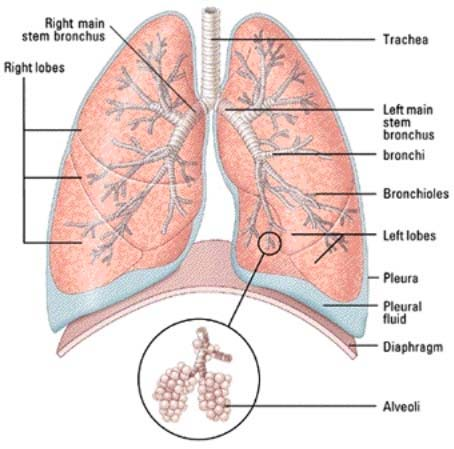
\includegraphics[width=0.5\textwidth]{../images/PF_I_1.jpg}
\caption{Diagram of lung anatomy}
\label{lung}
\end{figure}

The main role of the respiratory system is to provide oxygen (O\textsubscript{2}) to the body, while removing carbon dioxide (CO\textsubscript{2}) as waste. When air is breathed into the body, it travels through the oral cavities, throat, larynx, and trachea. It then enters the lungs, and after flowing through the bronchioles, it enters millions of alveoli. In the alveolar space, the gas exchange occurs through a simple diffusion process that is fueled by the partial pressure gradients of O\textsubscript{2}) and CO\textsubscript{2}). The air that has been inhaled has a higher concentration of O\textsubscript{2}) than that in the capillary blood. As a result, O\textsubscript{2}) travels down the pressure gradient and into the blood stream (Fig. \ref{exchange}). A similar process occurs with CO\textsubscript{2}) in the reverse direction.

\begin{figure}[h]
\centering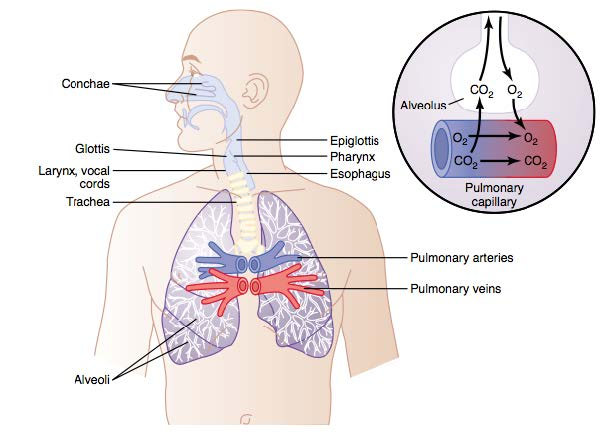
\includegraphics[width=0.6\textwidth]{../images/PF_I_2.jpg}
\caption{Pulmonary gas exchange}
\label{exchange}
\end{figure}

\textbf{Inspiration} (inhalation) is an active process, during which the diaphragm contracts and the rib cage expands to increase lung volume. As modeled by Boyle's Law, an increase in volume is correlated with a decrease in pressure. As the intrapulmonary pressure drops below atmospheric pressure (760 mmHg), a pressure gradient is formed and air flows into the lungs. At this point, gas exchange occurs. \textbf{Expiration} (exhalation), however, is mostly passive. The diaphragm and external intercostals relax as the abdominals contract. This causes a decrease in lung volume, an increase in intrapulmonary pressure, and the subsequent outflow of air.\\

Surface tension elastic forces of the alveolar membrane play a large role in the elastic recoil of the lungs. The area between the lung and thoracic wall, called the pleural cavity, contains fluid that helps lubricate movement of lungs within the cavity. The pressure within this space (negative pleural pressure) causes the volume of the lungs to increase and decrease with the expansion and contraction with the thoracic wall. The tendency of htel ungs to contract is called \textbf{elasticity}, and the lung's ability to increase in volume in response to an increase in pressure is called \textbf{compliance}.

\subsection*{Pulmonary Function Tests (Spirometry)}
Lifestyle, body type, disorders, and more can affect pulmonary function. These effects can be quantified for clinical use with a spirometer, which measures the volume and rate of air exhaled and inhaled.

\subsubsection*{Volumes and Capacities}

	\begin{table}[h]
	\centering
	\caption{Terms related to pulmonary function}
	\begin{tabular}[h!]{p{0.35\linewidth}p{0.15\linewidth}p{0.35\linewidth}}
	\toprule
	Term & Normal value & Definition\\
	\midrule
	Tidal Volume (TV) & ~500 mL & Volume of air during each normal breath\\\midrule
	Inspiratory Reserve Volume (IRV) & 3000 mL & Volume of air that can be forcefully inspired after tidal inspiration\\\midrule
	Expiratory Reserve Volume (ERV) & 1100 mL & Volume of air that can be forcefully expired after tidal expiration\\\midrule
	Residual Volume (RV) & 1200 mL & Volume of air left in lung following forced expiration (keeps the alveoli from collapsing)\\\midrule
	Inspiratory Capacity (IC) & TV + IRV & Maximum amount of air a person can breathe in after normal expiration\\\midrule
	Expiratory Capacity (EC) & TV + ERV & Maximum amount of air a person can breathe out after normal inspiration\\\midrule
	Functional Residual Capacity (FRC) & ERV + RV & Volume of air left in the lungs after normal expiration\\\midrule
	Vital Capacity (VC) & IRV + TV + ERV & Largest volume of air that can be expired after maximum inspiration\\\midrule
	Total Lung Capacity (TLC) & IRV + TV + ERV + RV & Maximum volume to which the lungs can be expanded\\
	\bottomrule
	\end{tabular}
	\label{volumes}
	\end{table}

\begin{figure}[h]
\centering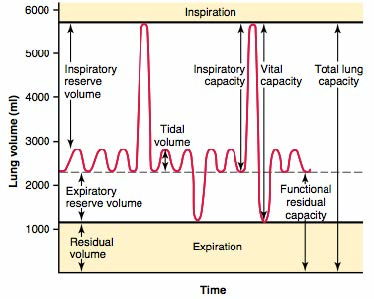
\includegraphics[width=0.5\textwidth]{../images/PF_I_3.jpg}
\caption{Pulmonary volumes and capacities}
\label{capacities}
\end{figure}

Pulmonary volumes can be determined by measuring volumes of inhaled and exhaled air, whereas capacities are derived form the sum of two or more volumes. Total lung capacity is the sum of all of these volumes and represents the maximum volume of air that the lungs can hold. Table \ref{volumes} and Fig. \ref{capacities} summarize these terms and their definitions.\\

\subsubsection*{Forced Expiratory Volume and Maximum Voluntary Ventilation}
In addition to examining lung volumes and capacities, quality of pulmonary function can also be determined by measuring pulmonary flow rates, or the airflow in and out of the lungs. Airflow resistance is a limiting factor in the ability of the lungs to efficiently move air in and out. Forced Expiratory Volume (FEV) and Maximum Voluntary Ventilation (MVV) are both indicative of such resistance. Table \ref{fvv} describes additional terms to pulmonary function.

	\begin{table}[h]
	\centering
	\caption{Additional terms related to pulmonary function}
	\begin{tabular}[h!]{p{0.35\linewidth}p{0.35\linewidth}}
	\toprule
	Term & Definition\\
	\midrule
	Forced Expiratory Volume (FEV) & Maximum amount of vital capacity air that can be expelled in a certain number of seconds (e.g. FEV\textsubscript{1}, FEV\textsubscript{1}, FEV\textsubscript{3})\\\midrule
	Forced Vital Capacity (FVC) & Maximum amount of air that a person can forcibly exhale after a maximal inhalation\\\midrule
	Maximum Voluntary Ventilation (MVV) & Maximum amount of air that can be inhaled and exhaled in one minute in L/min, breathing as quickly and deeply as possible. This combines volume and flow rates to assess overall pulmonary ventilation\\
	\bottomrule
	\end{tabular}
	\label{fvv}
	\end{table}

\subsection*{Clinical Relevance}
There are two main types of pulmonary disease:
\begin{itemize}
	\item \textbf{Restrictive} pulmonary diseases (such as pulmonary fibrosis) are characterized by normal airway resistance, but impaired respiratory movements because abnormalities in the lung tissue, pleura, chest wall, or neuromuscular machinery.
	\item \textbf{Obstructive} pulmonary diseases (such as asthma and COPD) are characterized by difficulty breathing due to increased airflow resistance.
\end{itemize}

\section*{Experiment 1}
\subsection*{Hardware and Software Setup}
\begin{enumerate}
	\item Plug the output line from the airflow transducer into channel 1 of the MP3X unit.
	\item Insert the filter into the inlet opening of the airflow transducer.
	\item Insert the calibration syringe into the other end of the filter (away from the airflow transducer) as seen in Fig. \ref{xdc}
		\begin{figure}[h]
	\centering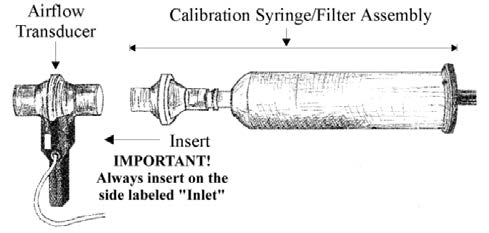
\includegraphics[width=0.6\textwidth]{../images/PF_I_4.jpg}
		\caption{Transducer setup}
		\label{xdc}
		\end{figure}
		
	\item Turn the MP3X unit on.
	\item From the desktop, open BIOPAC student lab 3.7. Selected L12 - PF 1.
\end{enumerate}

\subsection*{Calibration}
\begin{enumerate}
	\item Make sure to always handle this setup by holding the syringe, rather than the handle of the airflow transducer. This will ensure that the equipment remains properly aligned.
	\item Pull the syringe handle all the way out.
	\item Read the instructions below, then click the "Calibrate" button located int he upper left corner of the Setup window.
	\item During this recording, simply hold the assembly still and upright. Recording will end after 8 seconds and your screen should display a straight line.
	\item During this next part, you will push the syringe plunger in and out for a total of 5 cycles (push in and pull out for a total of 10 strokes). Pace yourself and try to achieve slow, smooth movement. Rest for a short time in between each plunge.
	\item Hold the syringe horizontally in one hand and use the other hand to plunge in and out completely.
	\item When you are ready to begin, click "OK" to start the calibration.
	\item When you finish calibrating, click "End Calibration." Your screen should resemble Fig. \ref{calibration}.
		\begin{figure}[h]
	\centering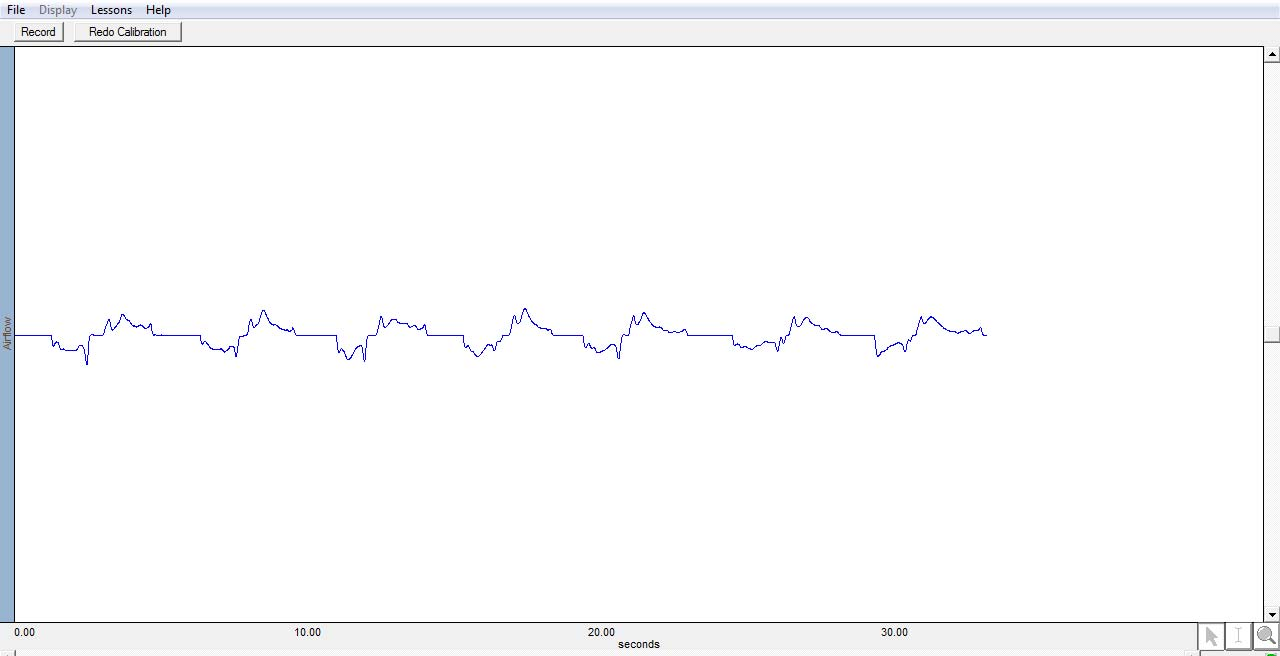
\includegraphics[width=0.6\textwidth]{../images/PF_I_5.jpg}
		\caption{Calibration procedure - plunge cycles}
		\label{calibration}
		\end{figure}
	
	\item If your calibration looks incorrect, click "Redo" and repeat the procedure.
\end{enumerate}

\subsection*{Test Procedure}
\begin{info}
	Keep the airflow transducer upright at all times during the experiment. If you start on an inhale, try to end on an exhale as this increases the accuracy of the airflow to volume calculation. Try not to look at the screen while recording as you may manipulate the results.
\end{info}
\begin{enumerate}
	\item Remove the calibration syringe and replace it with a disposable mouthpiece.
	\item Attach the nose clip to the subject's nose.
	\item Breathe normally through the mouthpiece for 20 seconds prior to the start of recording.
	\item Select "Record" when the subject is ready (Begin recording on an inhale).
	\item The subject must:\begin{enumerate}
		\item Continue breathing normally for 5 breath cycles.
		\item After a resting expiration, inhale as deeply as possible.
		\item Exhale to the point of normal resting expiration and continue breathing normally for 3-5 breaths.
		\item After a resting inspiration, maximally exhale (as completely as possible).
		\item Breathe normally for 5 breath cycles.
	\end{enumerate}
	
	\item When you are done recording, click on "Stop."
	\item If the data resembles Fig. \ref{example}, click "Done." Otherwise, click "Redo" and try again.
	
		\begin{figure}[h]
	\centering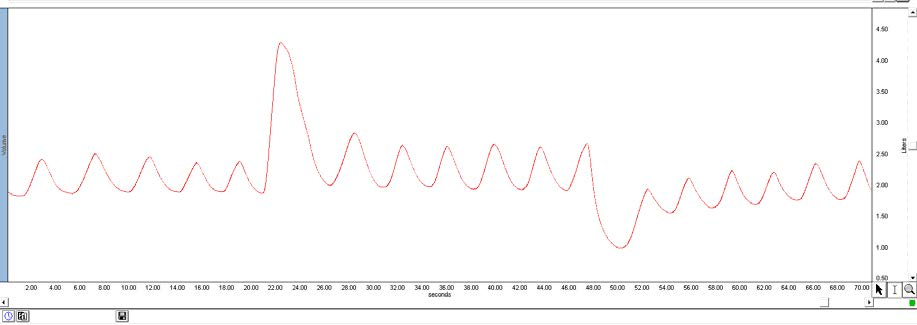
\includegraphics[width=0.6\textwidth]{../images/PF_I_6.jpg}
		\caption{Example pulmonary function data}
		\label{example}
		\end{figure}
	
	\begin{info}
		You will not be able to make additional measurements after this step, so make sure you have all the data needed.
	\end{info}
	\item From the pop-up window, select "Analyze current data file."
\end{enumerate}

\subsection*{Data Analysis}
\begin{enumerate}
	\item Complete the table in the handout. The tidal volume is the peak-to-peak volume measurement of a normal breath cycle. Calculate the Tidal Volume for three different breaths and take an average. Determine IRV, ERV, and VC for one breath
	\item Calculate the capacities listed in the table in the handout assuming a Residual Volume (RV) of 1 L.
	\item How would the volume measurements (TV, IRV, and ERV) change if data were collected after vigorous exercise?
	\item In this lab, equations for vital capacity (VC) were presented. Using the data provided, determine an equation for VC in the following form:\begin{equation}
		VC = b_0 + b_1x_1 + b_2x_2 + b_3x_3
	\end{equation}
	where $b_n$ is a regression parameter, $x_n$ is a variable (such as height). \textit{Hint: use a program that can perform multiple regression.}
	\item Qualitatively assess your equation. How do the variables (such as height) affect the VC? Is each of the parameters positively or negatively correlated to VC? What do the magnitude and sign of the regression parameters imply?
\end{enumerate}

\section*{Experiment 2}
\subsection*{Hardware and Software Setup}
\begin{enumerate}
	\item Remove the mouthpiece from the airflow transducer and insert the calibration syringe.
	\item From the desktop, open BIOPAC Student Lab v3.7 and select L13 - PF II.
	\item Follow the calibration procedure described in the previous section.
\end{enumerate}

\subsection*{Test Procedure}
\begin{info}
	Keep the airflow transducer upright at all times during the experiment. If you start on an inhale, try to end on an exhale as this increases the accuracy of the airflow to volume calibration. Try not to look at the screen while recording as you may manipulate the results.
\end{info}
\begin{enumerate}
	\item Remove the calibration syringe and replace it with a disposable mouthpiece.
	\item Attach a nose clip to the subject's nose.
	\item Breathe normally through the mouthpiece for 20 seconds prior to the start of recording.
	\item Select "Record FEV" when the subject is ready to start recording.
	\item The subject must:\begin{enumerate}
		\item Continue breathing normally for 3 breath cycles.
		\item After a resting expiration, inhale as deeply as possible.
		\item Hold their breath for an instant.
		\item Exhale as quickly and completely as possible.
	\end{enumerate}

	\item When you have collected your data, click "Stop."
	\item If the data does not resemble Fig. \ref{example_2}, click "Redo" and try again.
	\begin{figure}[h]
	\centering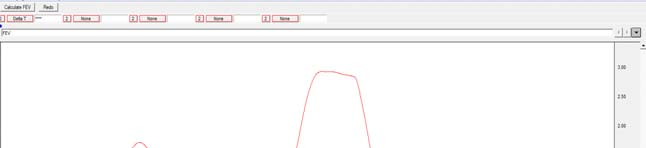
\includegraphics[width=0.6\textwidth]{../images/PF_I_7a.jpg}
	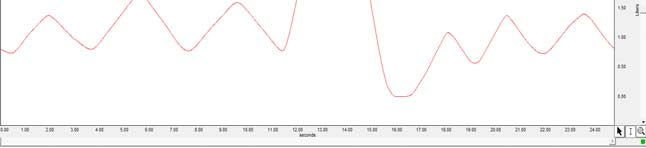
\includegraphics[width=0.6\textwidth]{../images/PF_I_7b.jpg}
		\caption{Example pulmonary function data}
		\label{example_2}
		\end{figure}
	
	\item Use the I-beam cursor to select the area of maximal exhale. Start at the exact point where the exhale begins and continue for 3 seconds (use delta T measurements to guarantee at least 3 seconds of data selection).
	\item Click on "Calculate FEV." This will automatically plot your data to show a cumulative expired volume over time,
	\item If you need to re-select the measurement area, click "Redo." Otherwise, click "Continue."
	\item Have the subject reapply nose clip, sit upright, and begin breathing through the airflow transducer.
	\item Select "Record MVV" when the subject is ready to start recording.
	\item The subject must:\begin{enumerate}
		\item Continue breathing normally into the airflow transducer for 5 breath cycles.
		\item Breath quickly and deeply for 12-15 seconds. Stop early if the subject feels dizzy.
		\item Breathe normally for 5 more cycles.
	\end{enumerate}
	
	\item Click on "Stop."
	\item Review the data on the screen. If the data does not resemble that in Fig. \ref{example_3}, click on "Redo." Otherwise, click "Done."
	\begin{figure}[h]
	\centering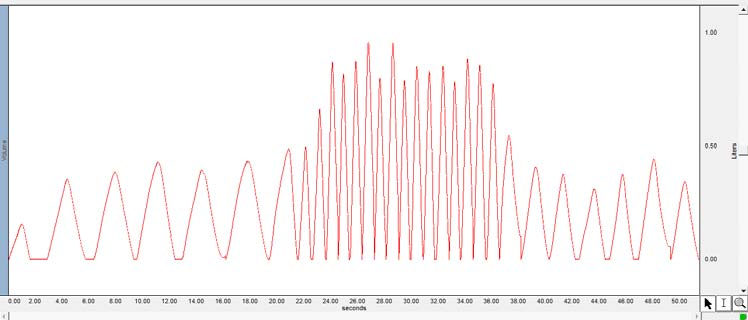
\includegraphics[width=0.6\textwidth]{../images/PF_I_8.jpg}
		\caption{Example pulmonary function data}
		\label{example_3}
		\end{figure}

	\item Select Analyze Current or Previous Data File to analyze data from the FEV or the MVV files, respectively. You can also access these files when you first open BIOPAC lessons, by selecting "Review Saved Data" instead of a specific lesson and looking for the folder where you saved your data.
\end{enumerate}

\subsection*{Data Analysis}
\begin{enumerate}
	\item Estimate the Vital Capacity using a p-p measurement.
	\item Calculate FEV\textsubscript{1}, FEV\textsubscript{2}, and FEV\textsubscript{3}.
	\item How do your calculated fractions of air expelled during the three listed time intervals compare with "normal" (average) values?
	\item Is it possible for a subject to have a vital capacity within normal range, but a value for FEV\textsubscript{1} below normal range? Explain.
	\item Using the data collected for the Maximal Voluntary Ventilation (MVV) measurements, calculate the respiratory rate (RR) over a 12-second interval. Do so by calculating the number of cycles in the 12-second interval and \textit{not} by highlighting the whole section and selecting Frequency.
	\item Complete the table in the handout with a measurement for each cycle. Complete only for the 12-second interval used above (the table may have more rows than you need). Calculate the average volume per cycle (AVPC).
	\item Calculate the MVV using the following formula:\begin{equation}
		MVV = AVPC \times RR
	\end{equation}
	
	\item Bronchodilator drugs open airways and clear mucous. How would these drugs affect the FEV and MVV measurements?
	\item MVV decreases with age. Why?
\end{enumerate}

\end{document}
